\section{Zielsetzung}
\label{sec:Zielsetzung}
In diesem Versuch wird die Suszeptibilität von Oxiden Seltener-Erd-Elemente experimentell bestimmt.

\section{Theorie}
\label{sec:Theorie}
\subsection{Theoretische Bestimmung der Suszeptibilität}
Der Zusammenhang von magnetischer Flussdichte $\vec{B}$ und magnetischer Feldstärke $\vec{H}$ ist gegeben durch
\begin{align*}
\vec{B} = \mu_0 \vec{H} + \vec{M},
\end{align*}
wobei $\mu_0$ die Induktionskonstante und $\vec{M}$ die Magnetisierung darstellen. Die
Magnetisierung $\vec{M}$, welche durch magnetische Momente in der Materie entsteht, ist eine von
$\vec{H}$ abhängige Größe:
\begin{equation}
\label{m}
\vec{M} = \mu_0 \chi \vec{H}.
\end{equation}
Hierbei ist $\chi$ die Suszeptibilität, welche wiederum von der magnetischen Feldstärke $\vec{H}$,
sowie von der Temperatur $T$ abhängt.

\noindent Im Gegensatz zum Diamagnetismus, welcher bei allen Materialien auftritt, ist der hier
betrachtete Paramagnetismus nicht bei jedem Element zu beobachten. Er tritt durch die Ausrichtung der 
magnetischen Moment relativ zu einem äußeren Magnetfeld auf. Die
Orientierung der magnetischen Momente wird durch die thermische Bewegung beeinflusst. Dies erklärt
die Temperaturabhängigkeit des Paramagnetismus. Paramagnetismus ist zu beobachten, wenn der
Drehimpuls des Atoms ungleich Null ist, da dieser mit den magnetischen Momenten gekoppelt ist.

\noindent Der Gesamtdrehimpuls $\vec{J}$ besteht aus dem Bahndrehimpuls der Elektronenhülle, dem
Spin der Elektronen, sowie dem Kerndrehimpuls, wobei letzterer bei Betrachtung des
Paramagnetismuses zu vernachlässigen ist. Wenn kein zu starkes äußeres Feld wirkt, setzt sich der
Gesamtdrehimpuls $\vec{J}$ aus der Summe des Gesamtbahndrehimpulses $\vec{L}$ und dem
Gesamtspin $\vec{S}$ zusammen:
\begin{align*}
\vec{J} = \vec{L} + \vec{S},
\end{align*}
wobei sich die Drehimpulse $\vec{L}$ und $\vec{S}$ aus der Summe der Einzeldrehimpulse
zusammensetzen. Für die magnetischen Momente der Drehimpulse $\vec{L}$ und $\vec{S}$ ergibt sich
aus quantenmechanischen Überlegungen:
\begin{align*}
\vec{\mu_\text{L}}=-\frac{\mu_\text{B}}{\hbar}\vec{L}, \\
\vec{\mu_\text{S}}=-g_\text{S}\frac{\mu_\text{B}}{\hbar}\vec{S},
\end{align*}
mit $\mu_\text{B}$ als Bohrsches Magneton und $g_\text{S}$ als gyromagnetisches Verhältnis des
freien Elektrons. Eine betragliche Betrachtung der Drehimpulse mit
\begin{align*}
\vert \vec{J}\vert= \sqrt{J(J+1)}\hbar, \\
\vert \vec{L}\vert= \sqrt{L(L+1)}\hbar, \\
\vert \vec{S}\vert= \sqrt{S(S+1)}\hbar
\end{align*}
liefert für die Beträge der magnetischen Momente:
\begin{align*}
\vert \vec{\mu_\text{L}}\vert = \mu_\text{B}\sqrt{S(S+1)}, \\
\vert \vec{\mu_\text{S}}\vert = g_\text{S}\mu_\text{B}\sqrt{S(S+1)}.
\end{align*}
Aus Abbildung \ref{fig:vektordiagramm} und geometrischen Beziehungen ergibt sich
\begin{align*}
\vert\vec{\mu_\text{J}}\vert = \vert\vec{\mu_\text{S}}\vert \cos\alpha + \vert\vec{\mu_\text{L}}\vert \cos\beta.
\end{align*}

\begin{figure}[H]
\centering
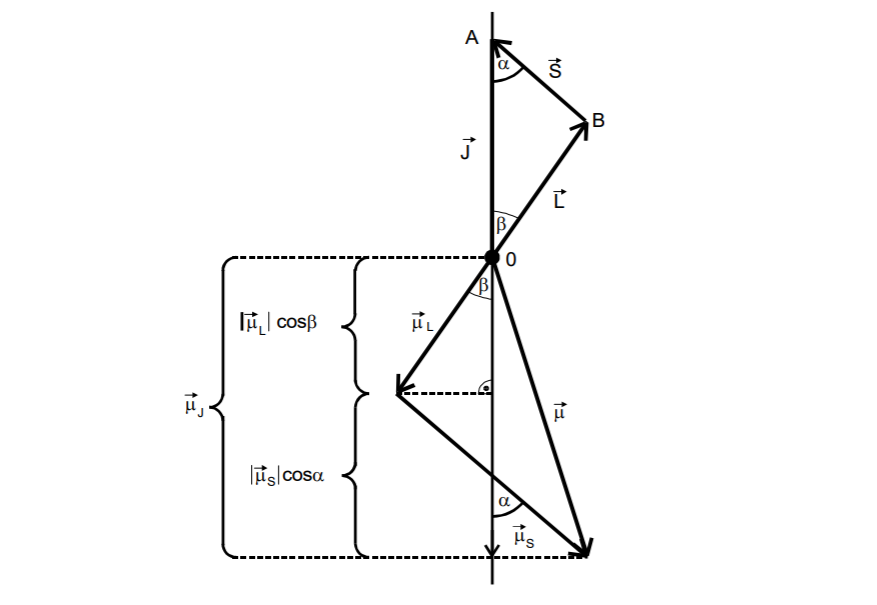
\includegraphics[scale=0.7]{vektor.png}
\caption{Vektordiagramm der Drehimpulsvektoren und magnetischen Momenten \cite{kent}.}
\label{fig:vektordiagramm}
\end{figure}

\noindent Aus der Quantenmechanik wird für $g_\text{S}$ eine Näherung mit dem Wert 2 angenommen, was
\begin{align*}
\vert\vec{\mu_\text{J}}\vert \approx \mu_\text{B}\sqrt{J(J+1)} \cdot \frac{3J(J+1)+(S(S+1)-L(L+1))}{2J(J+1)}
\end{align*}
zur Folge hat.
Dabei wird der Ausdruck
\begin{equation}
  \label{eqn:lande}
g_\text{J}:= \frac{3J(J+1)+(S(S+1)-L(L+1))}{2J(J+1)}
\end{equation}
als Landé-Faktor bezeichnet und führt zu der vereinfachten Schreibweise
\begin{align*}
\vert\vec{\mu_\text{J}}\vert \approx \mu_\text{B}g_\text{J}\sqrt{J(J+1)}.
\end{align*}

\noindent Desweiteren ist zu beachten, dass der Winkel zwischen der Richtung des äußeren
Magnetfelds und der Lage von $\vec{\mu_\text{J}}$ nicht beliebig ist, sondern die $z$-Komponente
von $\vec{\mu_\text{J}}$ ein ganzzahliges Vielfaches von $\mu_\text{B}g_\text{J}$ sein muss.
Dieser Effekt wird als Richtungsquantelung bezeichnet. Folglich ergibt sich hieraus für
\begin{align*}
\mu_{\text{J}_z} = - \mu_\text{B}g_\text{J}m,
\end{align*}
mit $m$ als Orientierungsquantenzahl und $2J+1$ möglichen Einstellungen mit je einer
zugehörigen potentiellen Energie. Mit dieser lässt sich auch die Magnetisierung $\vec{M}$ bestimmen.
Dazu wird die Häufigkeit der einzelnen Winkeleinstellungen benötigt und mit dem Betrag des
magnetischen Moments multipliziert. Anschließend wird über alle auftretenden Einstellungen summiert.
Somit ergibt sich nach Umformungen für die Suszeptibilität
\begin{equation}
\label{eqn:chi}
\chi = \frac{\mu_0\mu_\text{B}^2g_\text{J}^2NJ(J+1)}{3kT},
\end{equation}
mit $N$ als Anzahl der magnetischen Momente pro Volumeneinheit, $k$ als Boltzmann-Konstante und $T$
als Temperatur. Bei hohen Temperaturen $T$ ist die Suszeptibilität $\chi$ proportional zum
Kehrwert der Temperatur. Dieser Zusammenhang wird als Curiesche Gesetz des Paramagnetismus
bezeichnet.
Besonders stark ausgeprägt ist der Paramagnetismus bei Verbindungen, welche Ionen Seltener-Erd-Elemente
enthalten. Aus Gleichung~\ref{eqn:chi} folgt somit, dass ihre Elektronenhüllen große Drehimpulse
besitzen müssen. Dieser kommt durch die 4f-Elektronen zustande. Die Anordnung dieser Elektronen,
sowie der resultierende Gesamtdrehimpuls $\vec{J}$ werden durch die Hundschen Regeln bestimmt:
\begin{itemize}
\item Die einzelnen Spins $\vec{s_i}$ ergeben den maximalen Gesamtspin $\vec{S}=\sum \vec{s_i}$
 unter Berücksichtigung des Pauli-Prinzips.
\item Die Bahndrehimpulse $\vec{\ell_i}$ kombinieren zum maximalen Gesamtbahndrehimpuls
 $\vec{L}=\sum\vec{\ell_i}$ unter Beachtung der vorigen Regel und des Pauli-Prinzips.
\item Für den Gesamtdrehimpuls $\vec{J}$ ergibt sich $\vec{J}=\vec{L}-\vec{S}$ bei einer Schale, die
weniger als halb gefüllt ist und $\vec{J}=\vec{L}+\vec{S}$ sonst.
\end{itemize}
Das Pauli-Prinzip besagt, dass keine zwei Elektronen einer Hülle den gleichen Satz an
Quantenzahlen besitzen können.

\subsection{Experimentelle Bestimmung der Suszeptibilität}
Zur experimentellen Bestimmung der Suszeptibilität $\chi$ wird eine Brückenschaltung, wie in
Abbildung \ref{fig:schaltung} dargestellt, verwendet, welche zwei baugleiche Spulen enthält.
Hierbei ist wichtig, dass die Induktivität dieser Spulen möglichst gleich ist, da die
Induktivitätsdifferenz $\Delta L$ zwischen der Spule mit Probe und luftgefüllter Spule benötigt wird.
Bei dieser Brückenschaltung gibt es zwei Möglichkeiten der Messung. Bei der ersten wird die Brücke
zunächst abgeglichen. Dies bedeutet, dass theoretisch keine Brückenspannung $U_\text{Br}$ mehr zu
messen ist. Anschließend wird die Materialprobe in eine der Spulen eingeführt. Aus der nun
gemessenen Brückenspannung $U_\text{Br}$ kann für große Frequenzen die Suszeptibilität $\chi$ durch:
\begin{equation}
\label{eqn:chiex1}
\chi(\omega \rightarrow \infty)=4\frac{F U_\text{Br}}{A U_\text{Sp}},
\end{equation}
mit $F$ als Spulenquerschnittsfläche, $A$ als Probenquerschnittsfläche und $U_\text{Sp}$ als
Speisespannung, berechnet werden.

\noindent Bei der zweiten Methode wird zu Beginn ebenfalls die Brücke abgeglichen. Nachdem die Probe
in eine der beiden Spulen eingeführt wurde, wird die Brücke erneut abgeglichen. Aus der Differenz der
Abgleichbedingung zur Brückenspannung ergibt sich für die Suszeptibilität
\begin{equation}
\label{eqn:chiex2}
\chi=2\frac{\Delta R F}{R_3 A},
\end{equation}
mit $R_3$ als Widerstand am Potenziometer und $\Delta R$ als Differenz aus der Abgleichbedingung.

\begin{figure}[H]
\centering
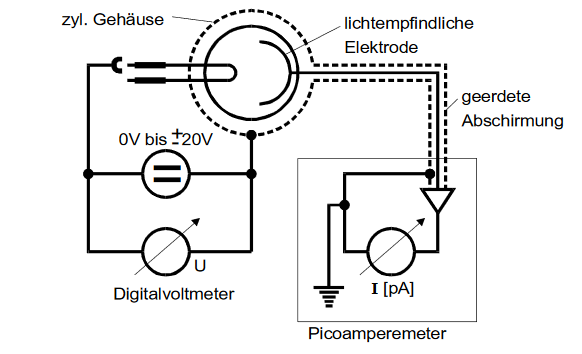
\includegraphics[scale=0.8]{schaltung.png}
\caption{Brückenschaltung zur Messung der Suszeptibilität \cite{kent}.}
\label{fig:schaltung}
\end{figure}
